% Created by tikzDevice version 0.10.1 on 2018-01-23 20:21:12
% !TEX encoding = UTF-8 Unicode
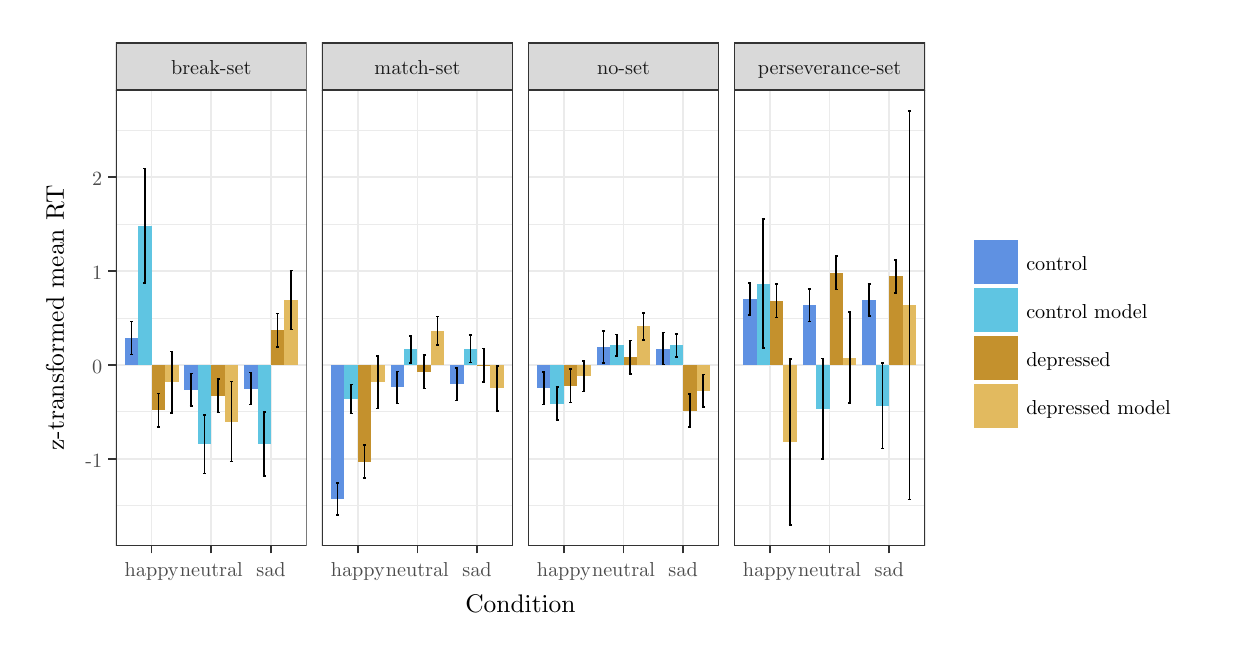
\begin{tikzpicture}[x=1pt,y=1pt]
\definecolor{fillColor}{RGB}{255,255,255}
\path[use as bounding box,fill=fillColor,fill opacity=0.00] (0,0) rectangle (433.62,216.81);
\begin{scope}
\path[clip] (  0.00,  0.00) rectangle (433.62,216.81);
\definecolor{drawColor}{RGB}{255,255,255}
\definecolor{fillColor}{RGB}{255,255,255}

\path[draw=drawColor,line width= 0.6pt,line join=round,line cap=round,fill=fillColor] (  0.00,  0.00) rectangle (433.62,216.81);
\end{scope}
\begin{scope}
\path[clip] ( 31.87, 29.59) rectangle (100.84,194.25);
\definecolor{fillColor}{RGB}{255,255,255}

\path[fill=fillColor] ( 31.87, 29.59) rectangle (100.84,194.25);
\definecolor{drawColor}{gray}{0.92}

\path[draw=drawColor,line width= 0.3pt,line join=round] ( 31.87, 44.03) --
	(100.84, 44.03);

\path[draw=drawColor,line width= 0.3pt,line join=round] ( 31.87, 77.97) --
	(100.84, 77.97);

\path[draw=drawColor,line width= 0.3pt,line join=round] ( 31.87,111.91) --
	(100.84,111.91);

\path[draw=drawColor,line width= 0.3pt,line join=round] ( 31.87,145.86) --
	(100.84,145.86);

\path[draw=drawColor,line width= 0.3pt,line join=round] ( 31.87,179.80) --
	(100.84,179.80);

\path[draw=drawColor,line width= 0.6pt,line join=round] ( 31.87, 61.00) --
	(100.84, 61.00);

\path[draw=drawColor,line width= 0.6pt,line join=round] ( 31.87, 94.94) --
	(100.84, 94.94);

\path[draw=drawColor,line width= 0.6pt,line join=round] ( 31.87,128.88) --
	(100.84,128.88);

\path[draw=drawColor,line width= 0.6pt,line join=round] ( 31.87,162.83) --
	(100.84,162.83);

\path[draw=drawColor,line width= 0.6pt,line join=round] ( 44.80, 29.59) --
	( 44.80,194.25);

\path[draw=drawColor,line width= 0.6pt,line join=round] ( 66.36, 29.59) --
	( 66.36,194.25);

\path[draw=drawColor,line width= 0.6pt,line join=round] ( 87.91, 29.59) --
	( 87.91,194.25);
\definecolor{fillColor}{RGB}{226,186,95}

\path[fill=fillColor] ( 49.65, 88.66) rectangle ( 54.50, 94.94);
\definecolor{fillColor}{RGB}{196,145,45}

\path[fill=fillColor] ( 44.80, 78.57) rectangle ( 49.65, 94.94);
\definecolor{fillColor}{RGB}{95,197,226}

\path[fill=fillColor] ( 39.95, 94.94) rectangle ( 44.80,145.25);
\definecolor{fillColor}{RGB}{95,145,226}

\path[fill=fillColor] ( 35.10, 94.94) rectangle ( 39.95,104.68);
\definecolor{fillColor}{RGB}{226,186,95}

\path[fill=fillColor] ( 71.21, 74.48) rectangle ( 76.06, 94.94);
\definecolor{fillColor}{RGB}{196,145,45}

\path[fill=fillColor] ( 66.36, 83.73) rectangle ( 71.21, 94.94);
\definecolor{fillColor}{RGB}{95,197,226}

\path[fill=fillColor] ( 61.51, 66.28) rectangle ( 66.36, 94.94);
\definecolor{fillColor}{RGB}{95,145,226}

\path[fill=fillColor] ( 56.66, 86.01) rectangle ( 61.51, 94.94);
\definecolor{fillColor}{RGB}{226,186,95}

\path[fill=fillColor] ( 92.76, 94.94) rectangle ( 97.61,118.42);
\definecolor{fillColor}{RGB}{196,145,45}

\path[fill=fillColor] ( 87.91, 94.94) rectangle ( 92.76,107.53);
\definecolor{fillColor}{RGB}{95,197,226}

\path[fill=fillColor] ( 83.06, 66.38) rectangle ( 87.91, 94.94);
\definecolor{fillColor}{RGB}{95,145,226}

\path[fill=fillColor] ( 78.21, 86.39) rectangle ( 83.06, 94.94);
\definecolor{drawColor}{RGB}{0,0,0}

\path[draw=drawColor,line width= 0.6pt,line join=round] ( 51.54, 99.75) --
	( 52.62, 99.75);

\path[draw=drawColor,line width= 0.6pt,line join=round] ( 52.08, 99.75) --
	( 52.08, 77.57);

\path[draw=drawColor,line width= 0.6pt,line join=round] ( 51.54, 77.57) --
	( 52.62, 77.57);

\path[draw=drawColor,line width= 0.6pt,line join=round] ( 46.69, 84.60) --
	( 47.77, 84.60);

\path[draw=drawColor,line width= 0.6pt,line join=round] ( 47.23, 84.60) --
	( 47.23, 72.55);

\path[draw=drawColor,line width= 0.6pt,line join=round] ( 46.69, 72.55) --
	( 47.77, 72.55);

\path[draw=drawColor,line width= 0.6pt,line join=round] ( 41.84,165.98) --
	( 42.92,165.98);

\path[draw=drawColor,line width= 0.6pt,line join=round] ( 42.38,165.98) --
	( 42.38,124.53);

\path[draw=drawColor,line width= 0.6pt,line join=round] ( 41.84,124.53) --
	( 42.92,124.53);

\path[draw=drawColor,line width= 0.6pt,line join=round] ( 36.99,110.63) --
	( 38.07,110.63);

\path[draw=drawColor,line width= 0.6pt,line join=round] ( 37.53,110.63) --
	( 37.53, 98.73);

\path[draw=drawColor,line width= 0.6pt,line join=round] ( 36.99, 98.73) --
	( 38.07, 98.73);

\path[draw=drawColor,line width= 0.6pt,line join=round] ( 73.09, 88.90) --
	( 74.17, 88.90);

\path[draw=drawColor,line width= 0.6pt,line join=round] ( 73.63, 88.90) --
	( 73.63, 60.06);

\path[draw=drawColor,line width= 0.6pt,line join=round] ( 73.09, 60.06) --
	( 74.17, 60.06);

\path[draw=drawColor,line width= 0.6pt,line join=round] ( 68.24, 89.74) --
	( 69.32, 89.74);

\path[draw=drawColor,line width= 0.6pt,line join=round] ( 68.78, 89.74) --
	( 68.78, 77.73);

\path[draw=drawColor,line width= 0.6pt,line join=round] ( 68.24, 77.73) --
	( 69.32, 77.73);

\path[draw=drawColor,line width= 0.6pt,line join=round] ( 63.39, 76.87) --
	( 64.47, 76.87);

\path[draw=drawColor,line width= 0.6pt,line join=round] ( 63.93, 76.87) --
	( 63.93, 55.69);

\path[draw=drawColor,line width= 0.6pt,line join=round] ( 63.39, 55.69) --
	( 64.47, 55.69);

\path[draw=drawColor,line width= 0.6pt,line join=round] ( 58.54, 91.80) --
	( 59.62, 91.80);

\path[draw=drawColor,line width= 0.6pt,line join=round] ( 59.08, 91.80) --
	( 59.08, 80.21);

\path[draw=drawColor,line width= 0.6pt,line join=round] ( 58.54, 80.21) --
	( 59.62, 80.21);

\path[draw=drawColor,line width= 0.6pt,line join=round] ( 94.65,129.05) --
	( 95.72,129.05);

\path[draw=drawColor,line width= 0.6pt,line join=round] ( 95.18,129.05) --
	( 95.18,107.80);

\path[draw=drawColor,line width= 0.6pt,line join=round] ( 94.65,107.80) --
	( 95.72,107.80);

\path[draw=drawColor,line width= 0.6pt,line join=round] ( 89.80,113.56) --
	( 90.87,113.56);

\path[draw=drawColor,line width= 0.6pt,line join=round] ( 90.33,113.56) --
	( 90.33,101.51);

\path[draw=drawColor,line width= 0.6pt,line join=round] ( 89.80,101.51) --
	( 90.87,101.51);

\path[draw=drawColor,line width= 0.6pt,line join=round] ( 84.95, 77.86) --
	( 86.02, 77.86);

\path[draw=drawColor,line width= 0.6pt,line join=round] ( 85.48, 77.86) --
	( 85.48, 54.91);

\path[draw=drawColor,line width= 0.6pt,line join=round] ( 84.95, 54.91) --
	( 86.02, 54.91);

\path[draw=drawColor,line width= 0.6pt,line join=round] ( 80.10, 92.19) --
	( 81.17, 92.19);

\path[draw=drawColor,line width= 0.6pt,line join=round] ( 80.64, 92.19) --
	( 80.64, 80.60);

\path[draw=drawColor,line width= 0.6pt,line join=round] ( 80.10, 80.60) --
	( 81.17, 80.60);
\definecolor{drawColor}{gray}{0.20}

\path[draw=drawColor,line width= 0.6pt,line join=round,line cap=round] ( 31.87, 29.59) rectangle (100.84,194.25);
\end{scope}
\begin{scope}
\path[clip] (106.34, 29.59) rectangle (175.31,194.25);
\definecolor{fillColor}{RGB}{255,255,255}

\path[fill=fillColor] (106.34, 29.59) rectangle (175.31,194.25);
\definecolor{drawColor}{gray}{0.92}

\path[draw=drawColor,line width= 0.3pt,line join=round] (106.34, 44.03) --
	(175.31, 44.03);

\path[draw=drawColor,line width= 0.3pt,line join=round] (106.34, 77.97) --
	(175.31, 77.97);

\path[draw=drawColor,line width= 0.3pt,line join=round] (106.34,111.91) --
	(175.31,111.91);

\path[draw=drawColor,line width= 0.3pt,line join=round] (106.34,145.86) --
	(175.31,145.86);

\path[draw=drawColor,line width= 0.3pt,line join=round] (106.34,179.80) --
	(175.31,179.80);

\path[draw=drawColor,line width= 0.6pt,line join=round] (106.34, 61.00) --
	(175.31, 61.00);

\path[draw=drawColor,line width= 0.6pt,line join=round] (106.34, 94.94) --
	(175.31, 94.94);

\path[draw=drawColor,line width= 0.6pt,line join=round] (106.34,128.88) --
	(175.31,128.88);

\path[draw=drawColor,line width= 0.6pt,line join=round] (106.34,162.83) --
	(175.31,162.83);

\path[draw=drawColor,line width= 0.6pt,line join=round] (119.27, 29.59) --
	(119.27,194.25);

\path[draw=drawColor,line width= 0.6pt,line join=round] (140.83, 29.59) --
	(140.83,194.25);

\path[draw=drawColor,line width= 0.6pt,line join=round] (162.38, 29.59) --
	(162.38,194.25);
\definecolor{fillColor}{RGB}{226,186,95}

\path[fill=fillColor] (124.12, 88.62) rectangle (128.97, 94.94);
\definecolor{fillColor}{RGB}{196,145,45}

\path[fill=fillColor] (119.27, 59.98) rectangle (124.12, 94.94);
\definecolor{fillColor}{RGB}{95,197,226}

\path[fill=fillColor] (114.42, 82.61) rectangle (119.27, 94.94);
\definecolor{fillColor}{RGB}{95,145,226}

\path[fill=fillColor] (109.57, 46.46) rectangle (114.42, 94.94);
\definecolor{fillColor}{RGB}{226,186,95}

\path[fill=fillColor] (145.68, 94.94) rectangle (150.53,107.37);
\definecolor{fillColor}{RGB}{196,145,45}

\path[fill=fillColor] (140.83, 92.48) rectangle (145.68, 94.94);
\definecolor{fillColor}{RGB}{95,197,226}

\path[fill=fillColor] (135.98, 94.94) rectangle (140.83,100.59);
\definecolor{fillColor}{RGB}{95,145,226}

\path[fill=fillColor] (131.13, 86.82) rectangle (135.98, 94.94);
\definecolor{fillColor}{RGB}{226,186,95}

\path[fill=fillColor] (167.23, 86.50) rectangle (172.08, 94.94);
\definecolor{fillColor}{RGB}{196,145,45}

\path[fill=fillColor] (162.38, 94.82) rectangle (167.23, 94.94);
\definecolor{fillColor}{RGB}{95,197,226}

\path[fill=fillColor] (157.53, 94.94) rectangle (162.38,100.80);
\definecolor{fillColor}{RGB}{95,145,226}

\path[fill=fillColor] (152.68, 87.93) rectangle (157.53, 94.94);
\definecolor{drawColor}{RGB}{0,0,0}

\path[draw=drawColor,line width= 0.6pt,line join=round] (126.01, 98.10) --
	(127.09, 98.10);

\path[draw=drawColor,line width= 0.6pt,line join=round] (126.55, 98.10) --
	(126.55, 79.15);

\path[draw=drawColor,line width= 0.6pt,line join=round] (126.01, 79.15) --
	(127.09, 79.15);

\path[draw=drawColor,line width= 0.6pt,line join=round] (121.16, 65.98) --
	(122.24, 65.98);

\path[draw=drawColor,line width= 0.6pt,line join=round] (121.70, 65.98) --
	(121.70, 53.97);

\path[draw=drawColor,line width= 0.6pt,line join=round] (121.16, 53.97) --
	(122.24, 53.97);

\path[draw=drawColor,line width= 0.6pt,line join=round] (116.31, 87.86) --
	(117.39, 87.86);

\path[draw=drawColor,line width= 0.6pt,line join=round] (116.85, 87.86) --
	(116.85, 77.36);

\path[draw=drawColor,line width= 0.6pt,line join=round] (116.31, 77.36) --
	(117.39, 77.36);

\path[draw=drawColor,line width= 0.6pt,line join=round] (111.46, 52.27) --
	(112.54, 52.27);

\path[draw=drawColor,line width= 0.6pt,line join=round] (112.00, 52.27) --
	(112.00, 40.64);

\path[draw=drawColor,line width= 0.6pt,line join=round] (111.46, 40.64) --
	(112.54, 40.64);

\path[draw=drawColor,line width= 0.6pt,line join=round] (147.56,112.48) --
	(148.64,112.48);

\path[draw=drawColor,line width= 0.6pt,line join=round] (148.10,112.48) --
	(148.10,102.26);

\path[draw=drawColor,line width= 0.6pt,line join=round] (147.56,102.26) --
	(148.64,102.26);

\path[draw=drawColor,line width= 0.6pt,line join=round] (142.71, 98.49) --
	(143.79, 98.49);

\path[draw=drawColor,line width= 0.6pt,line join=round] (143.25, 98.49) --
	(143.25, 86.47);

\path[draw=drawColor,line width= 0.6pt,line join=round] (142.71, 86.47) --
	(143.79, 86.47);

\path[draw=drawColor,line width= 0.6pt,line join=round] (137.86,105.51) --
	(138.94,105.51);

\path[draw=drawColor,line width= 0.6pt,line join=round] (138.40,105.51) --
	(138.40, 95.67);

\path[draw=drawColor,line width= 0.6pt,line join=round] (137.86, 95.67) --
	(138.94, 95.67);

\path[draw=drawColor,line width= 0.6pt,line join=round] (133.01, 92.61) --
	(134.09, 92.61);

\path[draw=drawColor,line width= 0.6pt,line join=round] (133.55, 92.61) --
	(133.55, 81.02);

\path[draw=drawColor,line width= 0.6pt,line join=round] (133.01, 81.02) --
	(134.09, 81.02);

\path[draw=drawColor,line width= 0.6pt,line join=round] (169.12, 94.67) --
	(170.19, 94.67);

\path[draw=drawColor,line width= 0.6pt,line join=round] (169.65, 94.67) --
	(169.65, 78.33);

\path[draw=drawColor,line width= 0.6pt,line join=round] (169.12, 78.33) --
	(170.19, 78.33);

\path[draw=drawColor,line width= 0.6pt,line join=round] (164.27,100.83) --
	(165.34,100.83);

\path[draw=drawColor,line width= 0.6pt,line join=round] (164.80,100.83) --
	(164.80, 88.82);

\path[draw=drawColor,line width= 0.6pt,line join=round] (164.27, 88.82) --
	(165.34, 88.82);

\path[draw=drawColor,line width= 0.6pt,line join=round] (159.42,105.82) --
	(160.49,105.82);

\path[draw=drawColor,line width= 0.6pt,line join=round] (159.96,105.82) --
	(159.96, 95.78);

\path[draw=drawColor,line width= 0.6pt,line join=round] (159.42, 95.78) --
	(160.49, 95.78);

\path[draw=drawColor,line width= 0.6pt,line join=round] (154.57, 93.73) --
	(155.64, 93.73);

\path[draw=drawColor,line width= 0.6pt,line join=round] (155.11, 93.73) --
	(155.11, 82.14);

\path[draw=drawColor,line width= 0.6pt,line join=round] (154.57, 82.14) --
	(155.64, 82.14);
\definecolor{drawColor}{gray}{0.20}

\path[draw=drawColor,line width= 0.6pt,line join=round,line cap=round] (106.34, 29.59) rectangle (175.31,194.25);
\end{scope}
\begin{scope}
\path[clip] (180.81, 29.59) rectangle (249.78,194.25);
\definecolor{fillColor}{RGB}{255,255,255}

\path[fill=fillColor] (180.81, 29.59) rectangle (249.78,194.25);
\definecolor{drawColor}{gray}{0.92}

\path[draw=drawColor,line width= 0.3pt,line join=round] (180.81, 44.03) --
	(249.78, 44.03);

\path[draw=drawColor,line width= 0.3pt,line join=round] (180.81, 77.97) --
	(249.78, 77.97);

\path[draw=drawColor,line width= 0.3pt,line join=round] (180.81,111.91) --
	(249.78,111.91);

\path[draw=drawColor,line width= 0.3pt,line join=round] (180.81,145.86) --
	(249.78,145.86);

\path[draw=drawColor,line width= 0.3pt,line join=round] (180.81,179.80) --
	(249.78,179.80);

\path[draw=drawColor,line width= 0.6pt,line join=round] (180.81, 61.00) --
	(249.78, 61.00);

\path[draw=drawColor,line width= 0.6pt,line join=round] (180.81, 94.94) --
	(249.78, 94.94);

\path[draw=drawColor,line width= 0.6pt,line join=round] (180.81,128.88) --
	(249.78,128.88);

\path[draw=drawColor,line width= 0.6pt,line join=round] (180.81,162.83) --
	(249.78,162.83);

\path[draw=drawColor,line width= 0.6pt,line join=round] (193.74, 29.59) --
	(193.74,194.25);

\path[draw=drawColor,line width= 0.6pt,line join=round] (215.30, 29.59) --
	(215.30,194.25);

\path[draw=drawColor,line width= 0.6pt,line join=round] (236.85, 29.59) --
	(236.85,194.25);
\definecolor{fillColor}{RGB}{226,186,95}

\path[fill=fillColor] (198.59, 90.82) rectangle (203.44, 94.94);
\definecolor{fillColor}{RGB}{196,145,45}

\path[fill=fillColor] (193.74, 87.39) rectangle (198.59, 94.94);
\definecolor{fillColor}{RGB}{95,197,226}

\path[fill=fillColor] (188.89, 80.96) rectangle (193.74, 94.94);
\definecolor{fillColor}{RGB}{95,145,226}

\path[fill=fillColor] (184.05, 86.51) rectangle (188.89, 94.94);
\definecolor{fillColor}{RGB}{226,186,95}

\path[fill=fillColor] (220.15, 94.94) rectangle (225.00,108.90);
\definecolor{fillColor}{RGB}{196,145,45}

\path[fill=fillColor] (215.30, 94.94) rectangle (220.15, 97.79);
\definecolor{fillColor}{RGB}{95,197,226}

\path[fill=fillColor] (210.45, 94.94) rectangle (215.30,102.11);
\definecolor{fillColor}{RGB}{95,145,226}

\path[fill=fillColor] (205.60, 94.94) rectangle (210.45,101.33);
\definecolor{fillColor}{RGB}{226,186,95}

\path[fill=fillColor] (241.70, 85.66) rectangle (246.55, 94.94);
\definecolor{fillColor}{RGB}{196,145,45}

\path[fill=fillColor] (236.85, 78.46) rectangle (241.70, 94.94);
\definecolor{fillColor}{RGB}{95,197,226}

\path[fill=fillColor] (232.00, 94.94) rectangle (236.85,101.99);
\definecolor{fillColor}{RGB}{95,145,226}

\path[fill=fillColor] (227.15, 94.94) rectangle (232.00,100.83);
\definecolor{drawColor}{RGB}{0,0,0}

\path[draw=drawColor,line width= 0.6pt,line join=round] (200.48, 96.26) --
	(201.56, 96.26);

\path[draw=drawColor,line width= 0.6pt,line join=round] (201.02, 96.26) --
	(201.02, 85.38);

\path[draw=drawColor,line width= 0.6pt,line join=round] (200.48, 85.38) --
	(201.56, 85.38);

\path[draw=drawColor,line width= 0.6pt,line join=round] (195.63, 93.40) --
	(196.71, 93.40);

\path[draw=drawColor,line width= 0.6pt,line join=round] (196.17, 93.40) --
	(196.17, 81.38);

\path[draw=drawColor,line width= 0.6pt,line join=round] (195.63, 81.38) --
	(196.71, 81.38);

\path[draw=drawColor,line width= 0.6pt,line join=round] (190.78, 86.87) --
	(191.86, 86.87);

\path[draw=drawColor,line width= 0.6pt,line join=round] (191.32, 86.87) --
	(191.32, 75.06);

\path[draw=drawColor,line width= 0.6pt,line join=round] (190.78, 75.06) --
	(191.86, 75.06);

\path[draw=drawColor,line width= 0.6pt,line join=round] (185.93, 92.32) --
	(187.01, 92.32);

\path[draw=drawColor,line width= 0.6pt,line join=round] (186.47, 92.32) --
	(186.47, 80.69);

\path[draw=drawColor,line width= 0.6pt,line join=round] (185.93, 80.69) --
	(187.01, 80.69);

\path[draw=drawColor,line width= 0.6pt,line join=round] (222.03,113.78) --
	(223.11,113.78);

\path[draw=drawColor,line width= 0.6pt,line join=round] (222.57,113.78) --
	(222.57,104.03);

\path[draw=drawColor,line width= 0.6pt,line join=round] (222.03,104.03) --
	(223.11,104.03);

\path[draw=drawColor,line width= 0.6pt,line join=round] (217.18,103.82) --
	(218.26,103.82);

\path[draw=drawColor,line width= 0.6pt,line join=round] (217.72,103.82) --
	(217.72, 91.76);

\path[draw=drawColor,line width= 0.6pt,line join=round] (217.18, 91.76) --
	(218.26, 91.76);

\path[draw=drawColor,line width= 0.6pt,line join=round] (212.33,105.98) --
	(213.41,105.98);

\path[draw=drawColor,line width= 0.6pt,line join=round] (212.87,105.98) --
	(212.87, 98.25);

\path[draw=drawColor,line width= 0.6pt,line join=round] (212.33, 98.25) --
	(213.41, 98.25);

\path[draw=drawColor,line width= 0.6pt,line join=round] (207.48,107.13) --
	(208.56,107.13);

\path[draw=drawColor,line width= 0.6pt,line join=round] (208.02,107.13) --
	(208.02, 95.54);

\path[draw=drawColor,line width= 0.6pt,line join=round] (207.48, 95.54) --
	(208.56, 95.54);

\path[draw=drawColor,line width= 0.6pt,line join=round] (243.59, 91.54) --
	(244.66, 91.54);

\path[draw=drawColor,line width= 0.6pt,line join=round] (244.12, 91.54) --
	(244.12, 79.77);

\path[draw=drawColor,line width= 0.6pt,line join=round] (243.59, 79.77) --
	(244.66, 79.77);

\path[draw=drawColor,line width= 0.6pt,line join=round] (238.74, 84.47) --
	(239.81, 84.47);

\path[draw=drawColor,line width= 0.6pt,line join=round] (239.28, 84.47) --
	(239.28, 72.45);

\path[draw=drawColor,line width= 0.6pt,line join=round] (238.74, 72.45) --
	(239.81, 72.45);

\path[draw=drawColor,line width= 0.6pt,line join=round] (233.89,106.08) --
	(234.96,106.08);

\path[draw=drawColor,line width= 0.6pt,line join=round] (234.43,106.08) --
	(234.43, 97.91);

\path[draw=drawColor,line width= 0.6pt,line join=round] (233.89, 97.91) --
	(234.96, 97.91);

\path[draw=drawColor,line width= 0.6pt,line join=round] (229.04,106.63) --
	(230.12,106.63);

\path[draw=drawColor,line width= 0.6pt,line join=round] (229.58,106.63) --
	(229.58, 95.04);

\path[draw=drawColor,line width= 0.6pt,line join=round] (229.04, 95.04) --
	(230.12, 95.04);
\definecolor{drawColor}{gray}{0.20}

\path[draw=drawColor,line width= 0.6pt,line join=round,line cap=round] (180.81, 29.59) rectangle (249.78,194.25);
\end{scope}
\begin{scope}
\path[clip] (255.28, 29.59) rectangle (324.25,194.25);
\definecolor{fillColor}{RGB}{255,255,255}

\path[fill=fillColor] (255.28, 29.59) rectangle (324.25,194.25);
\definecolor{drawColor}{gray}{0.92}

\path[draw=drawColor,line width= 0.3pt,line join=round] (255.28, 44.03) --
	(324.25, 44.03);

\path[draw=drawColor,line width= 0.3pt,line join=round] (255.28, 77.97) --
	(324.25, 77.97);

\path[draw=drawColor,line width= 0.3pt,line join=round] (255.28,111.91) --
	(324.25,111.91);

\path[draw=drawColor,line width= 0.3pt,line join=round] (255.28,145.86) --
	(324.25,145.86);

\path[draw=drawColor,line width= 0.3pt,line join=round] (255.28,179.80) --
	(324.25,179.80);

\path[draw=drawColor,line width= 0.6pt,line join=round] (255.28, 61.00) --
	(324.25, 61.00);

\path[draw=drawColor,line width= 0.6pt,line join=round] (255.28, 94.94) --
	(324.25, 94.94);

\path[draw=drawColor,line width= 0.6pt,line join=round] (255.28,128.88) --
	(324.25,128.88);

\path[draw=drawColor,line width= 0.6pt,line join=round] (255.28,162.83) --
	(324.25,162.83);

\path[draw=drawColor,line width= 0.6pt,line join=round] (268.21, 29.59) --
	(268.21,194.25);

\path[draw=drawColor,line width= 0.6pt,line join=round] (289.77, 29.59) --
	(289.77,194.25);

\path[draw=drawColor,line width= 0.6pt,line join=round] (311.32, 29.59) --
	(311.32,194.25);
\definecolor{fillColor}{RGB}{226,186,95}

\path[fill=fillColor] (273.06, 67.11) rectangle (277.91, 94.94);
\definecolor{fillColor}{RGB}{196,145,45}

\path[fill=fillColor] (268.21, 94.94) rectangle (273.06,118.08);
\definecolor{fillColor}{RGB}{95,197,226}

\path[fill=fillColor] (263.37, 94.94) rectangle (268.21,124.27);
\definecolor{fillColor}{RGB}{95,145,226}

\path[fill=fillColor] (258.52, 94.94) rectangle (263.37,118.81);
\definecolor{fillColor}{RGB}{226,186,95}

\path[fill=fillColor] (294.62, 94.94) rectangle (299.47, 97.57);
\definecolor{fillColor}{RGB}{196,145,45}

\path[fill=fillColor] (289.77, 94.94) rectangle (294.62,128.25);
\definecolor{fillColor}{RGB}{95,197,226}

\path[fill=fillColor] (284.92, 79.04) rectangle (289.77, 94.94);
\definecolor{fillColor}{RGB}{95,145,226}

\path[fill=fillColor] (280.07, 94.94) rectangle (284.92,116.47);
\definecolor{fillColor}{RGB}{226,186,95}

\path[fill=fillColor] (316.17, 94.94) rectangle (321.02,116.56);
\definecolor{fillColor}{RGB}{196,145,45}

\path[fill=fillColor] (311.32, 94.94) rectangle (316.17,126.94);
\definecolor{fillColor}{RGB}{95,197,226}

\path[fill=fillColor] (306.47, 80.15) rectangle (311.32, 94.94);
\definecolor{fillColor}{RGB}{95,145,226}

\path[fill=fillColor] (301.62, 94.94) rectangle (306.47,118.39);
\definecolor{drawColor}{RGB}{0,0,0}

\path[draw=drawColor,line width= 0.6pt,line join=round] (274.95, 97.15) --
	(276.03, 97.15);

\path[draw=drawColor,line width= 0.6pt,line join=round] (275.49, 97.15) --
	(275.49, 37.07);

\path[draw=drawColor,line width= 0.6pt,line join=round] (274.95, 37.07) --
	(276.03, 37.07);

\path[draw=drawColor,line width= 0.6pt,line join=round] (270.10,124.09) --
	(271.18,124.09);

\path[draw=drawColor,line width= 0.6pt,line join=round] (270.64,124.09) --
	(270.64,112.08);

\path[draw=drawColor,line width= 0.6pt,line join=round] (270.10,112.08) --
	(271.18,112.08);

\path[draw=drawColor,line width= 0.6pt,line join=round] (265.25,147.60) --
	(266.33,147.60);

\path[draw=drawColor,line width= 0.6pt,line join=round] (265.79,147.60) --
	(265.79,100.94);

\path[draw=drawColor,line width= 0.6pt,line join=round] (265.25,100.94) --
	(266.33,100.94);

\path[draw=drawColor,line width= 0.6pt,line join=round] (260.40,124.61) --
	(261.48,124.61);

\path[draw=drawColor,line width= 0.6pt,line join=round] (260.94,124.61) --
	(260.94,113.02);

\path[draw=drawColor,line width= 0.6pt,line join=round] (260.40,113.02) --
	(261.48,113.02);

\path[draw=drawColor,line width= 0.6pt,line join=round] (296.50,113.99) --
	(297.58,113.99);

\path[draw=drawColor,line width= 0.6pt,line join=round] (297.04,113.99) --
	(297.04, 81.14);

\path[draw=drawColor,line width= 0.6pt,line join=round] (296.50, 81.14) --
	(297.58, 81.14);

\path[draw=drawColor,line width= 0.6pt,line join=round] (291.65,134.26) --
	(292.73,134.26);

\path[draw=drawColor,line width= 0.6pt,line join=round] (292.19,134.26) --
	(292.19,122.24);

\path[draw=drawColor,line width= 0.6pt,line join=round] (291.65,122.24) --
	(292.73,122.24);

\path[draw=drawColor,line width= 0.6pt,line join=round] (286.80, 97.23) --
	(287.88, 97.23);

\path[draw=drawColor,line width= 0.6pt,line join=round] (287.34, 97.23) --
	(287.34, 60.85);

\path[draw=drawColor,line width= 0.6pt,line join=round] (286.80, 60.85) --
	(287.88, 60.85);

\path[draw=drawColor,line width= 0.6pt,line join=round] (281.95,122.26) --
	(283.03,122.26);

\path[draw=drawColor,line width= 0.6pt,line join=round] (282.49,122.26) --
	(282.49,110.67);

\path[draw=drawColor,line width= 0.6pt,line join=round] (281.95,110.67) --
	(283.03,110.67);

\path[draw=drawColor,line width= 0.6pt,line join=round] (318.06,186.76) --
	(319.13,186.76);

\path[draw=drawColor,line width= 0.6pt,line join=round] (318.60,186.76) --
	(318.60, 46.36);

\path[draw=drawColor,line width= 0.6pt,line join=round] (318.06, 46.36) --
	(319.13, 46.36);

\path[draw=drawColor,line width= 0.6pt,line join=round] (313.21,132.95) --
	(314.28,132.95);

\path[draw=drawColor,line width= 0.6pt,line join=round] (313.75,132.95) --
	(313.75,120.93);

\path[draw=drawColor,line width= 0.6pt,line join=round] (313.21,120.93) --
	(314.28,120.93);

\path[draw=drawColor,line width= 0.6pt,line join=round] (308.36, 95.58) --
	(309.44, 95.58);

\path[draw=drawColor,line width= 0.6pt,line join=round] (308.90, 95.58) --
	(308.90, 64.73);

\path[draw=drawColor,line width= 0.6pt,line join=round] (308.36, 64.73) --
	(309.44, 64.73);

\path[draw=drawColor,line width= 0.6pt,line join=round] (303.51,124.19) --
	(304.59,124.19);

\path[draw=drawColor,line width= 0.6pt,line join=round] (304.05,124.19) --
	(304.05,112.60);

\path[draw=drawColor,line width= 0.6pt,line join=round] (303.51,112.60) --
	(304.59,112.60);
\definecolor{drawColor}{gray}{0.20}

\path[draw=drawColor,line width= 0.6pt,line join=round,line cap=round] (255.28, 29.59) rectangle (324.25,194.25);
\end{scope}
\begin{scope}
\path[clip] ( 31.87,194.25) rectangle (100.84,211.31);
\definecolor{drawColor}{gray}{0.20}
\definecolor{fillColor}{gray}{0.85}

\path[draw=drawColor,line width= 0.6pt,line join=round,line cap=round,fill=fillColor] ( 31.87,194.25) rectangle (100.84,211.31);
\definecolor{drawColor}{gray}{0.10}

\node[text=drawColor,anchor=base,inner sep=0pt, outer sep=0pt, scale=  0.73] at ( 66.36,199.75) {break-set};
\end{scope}
\begin{scope}
\path[clip] (106.34,194.25) rectangle (175.31,211.31);
\definecolor{drawColor}{gray}{0.20}
\definecolor{fillColor}{gray}{0.85}

\path[draw=drawColor,line width= 0.6pt,line join=round,line cap=round,fill=fillColor] (106.34,194.25) rectangle (175.31,211.31);
\definecolor{drawColor}{gray}{0.10}

\node[text=drawColor,anchor=base,inner sep=0pt, outer sep=0pt, scale=  0.73] at (140.83,199.75) {match-set};
\end{scope}
\begin{scope}
\path[clip] (180.81,194.25) rectangle (249.78,211.31);
\definecolor{drawColor}{gray}{0.20}
\definecolor{fillColor}{gray}{0.85}

\path[draw=drawColor,line width= 0.6pt,line join=round,line cap=round,fill=fillColor] (180.81,194.25) rectangle (249.78,211.31);
\definecolor{drawColor}{gray}{0.10}

\node[text=drawColor,anchor=base,inner sep=0pt, outer sep=0pt, scale=  0.73] at (215.30,199.75) {no-set};
\end{scope}
\begin{scope}
\path[clip] (255.28,194.25) rectangle (324.25,211.31);
\definecolor{drawColor}{gray}{0.20}
\definecolor{fillColor}{gray}{0.85}

\path[draw=drawColor,line width= 0.6pt,line join=round,line cap=round,fill=fillColor] (255.28,194.25) rectangle (324.25,211.31);
\definecolor{drawColor}{gray}{0.10}

\node[text=drawColor,anchor=base,inner sep=0pt, outer sep=0pt, scale=  0.73] at (289.77,199.75) {perseverance-set};
\end{scope}
\begin{scope}
\path[clip] (  0.00,  0.00) rectangle (433.62,216.81);
\definecolor{drawColor}{gray}{0.20}

\path[draw=drawColor,line width= 0.6pt,line join=round] ( 44.80, 26.84) --
	( 44.80, 29.59);

\path[draw=drawColor,line width= 0.6pt,line join=round] ( 66.36, 26.84) --
	( 66.36, 29.59);

\path[draw=drawColor,line width= 0.6pt,line join=round] ( 87.91, 26.84) --
	( 87.91, 29.59);
\end{scope}
\begin{scope}
\path[clip] (  0.00,  0.00) rectangle (433.62,216.81);
\definecolor{drawColor}{gray}{0.30}

\node[text=drawColor,anchor=base,inner sep=0pt, outer sep=0pt, scale=  0.73] at ( 44.80, 18.58) {happy};

\node[text=drawColor,anchor=base,inner sep=0pt, outer sep=0pt, scale=  0.73] at ( 66.36, 18.58) {neutral};

\node[text=drawColor,anchor=base,inner sep=0pt, outer sep=0pt, scale=  0.73] at ( 87.91, 18.58) {sad};
\end{scope}
\begin{scope}
\path[clip] (  0.00,  0.00) rectangle (433.62,216.81);
\definecolor{drawColor}{gray}{0.20}

\path[draw=drawColor,line width= 0.6pt,line join=round] (119.27, 26.84) --
	(119.27, 29.59);

\path[draw=drawColor,line width= 0.6pt,line join=round] (140.83, 26.84) --
	(140.83, 29.59);

\path[draw=drawColor,line width= 0.6pt,line join=round] (162.38, 26.84) --
	(162.38, 29.59);
\end{scope}
\begin{scope}
\path[clip] (  0.00,  0.00) rectangle (433.62,216.81);
\definecolor{drawColor}{gray}{0.30}

\node[text=drawColor,anchor=base,inner sep=0pt, outer sep=0pt, scale=  0.73] at (119.27, 18.58) {happy};

\node[text=drawColor,anchor=base,inner sep=0pt, outer sep=0pt, scale=  0.73] at (140.83, 18.58) {neutral};

\node[text=drawColor,anchor=base,inner sep=0pt, outer sep=0pt, scale=  0.73] at (162.38, 18.58) {sad};
\end{scope}
\begin{scope}
\path[clip] (  0.00,  0.00) rectangle (433.62,216.81);
\definecolor{drawColor}{gray}{0.20}

\path[draw=drawColor,line width= 0.6pt,line join=round] (193.74, 26.84) --
	(193.74, 29.59);

\path[draw=drawColor,line width= 0.6pt,line join=round] (215.30, 26.84) --
	(215.30, 29.59);

\path[draw=drawColor,line width= 0.6pt,line join=round] (236.85, 26.84) --
	(236.85, 29.59);
\end{scope}
\begin{scope}
\path[clip] (  0.00,  0.00) rectangle (433.62,216.81);
\definecolor{drawColor}{gray}{0.30}

\node[text=drawColor,anchor=base,inner sep=0pt, outer sep=0pt, scale=  0.73] at (193.74, 18.58) {happy};

\node[text=drawColor,anchor=base,inner sep=0pt, outer sep=0pt, scale=  0.73] at (215.30, 18.58) {neutral};

\node[text=drawColor,anchor=base,inner sep=0pt, outer sep=0pt, scale=  0.73] at (236.85, 18.58) {sad};
\end{scope}
\begin{scope}
\path[clip] (  0.00,  0.00) rectangle (433.62,216.81);
\definecolor{drawColor}{gray}{0.20}

\path[draw=drawColor,line width= 0.6pt,line join=round] (268.21, 26.84) --
	(268.21, 29.59);

\path[draw=drawColor,line width= 0.6pt,line join=round] (289.77, 26.84) --
	(289.77, 29.59);

\path[draw=drawColor,line width= 0.6pt,line join=round] (311.32, 26.84) --
	(311.32, 29.59);
\end{scope}
\begin{scope}
\path[clip] (  0.00,  0.00) rectangle (433.62,216.81);
\definecolor{drawColor}{gray}{0.30}

\node[text=drawColor,anchor=base,inner sep=0pt, outer sep=0pt, scale=  0.73] at (268.21, 18.58) {happy};

\node[text=drawColor,anchor=base,inner sep=0pt, outer sep=0pt, scale=  0.73] at (289.77, 18.58) {neutral};

\node[text=drawColor,anchor=base,inner sep=0pt, outer sep=0pt, scale=  0.73] at (311.32, 18.58) {sad};
\end{scope}
\begin{scope}
\path[clip] (  0.00,  0.00) rectangle (433.62,216.81);
\definecolor{drawColor}{gray}{0.30}

\node[text=drawColor,anchor=base east,inner sep=0pt, outer sep=0pt, scale=  0.73] at ( 26.92, 57.97) {-1};

\node[text=drawColor,anchor=base east,inner sep=0pt, outer sep=0pt, scale=  0.73] at ( 26.92, 91.91) {0};

\node[text=drawColor,anchor=base east,inner sep=0pt, outer sep=0pt, scale=  0.73] at ( 26.92,125.85) {1};

\node[text=drawColor,anchor=base east,inner sep=0pt, outer sep=0pt, scale=  0.73] at ( 26.92,159.80) {2};
\end{scope}
\begin{scope}
\path[clip] (  0.00,  0.00) rectangle (433.62,216.81);
\definecolor{drawColor}{gray}{0.20}

\path[draw=drawColor,line width= 0.6pt,line join=round] ( 29.12, 61.00) --
	( 31.87, 61.00);

\path[draw=drawColor,line width= 0.6pt,line join=round] ( 29.12, 94.94) --
	( 31.87, 94.94);

\path[draw=drawColor,line width= 0.6pt,line join=round] ( 29.12,128.88) --
	( 31.87,128.88);

\path[draw=drawColor,line width= 0.6pt,line join=round] ( 29.12,162.83) --
	( 31.87,162.83);
\end{scope}
\begin{scope}
\path[clip] (  0.00,  0.00) rectangle (433.62,216.81);
\definecolor{drawColor}{RGB}{0,0,0}

\node[text=drawColor,anchor=base,inner sep=0pt, outer sep=0pt, scale=  0.92] at (178.06,  5.50) {Condition};
\end{scope}
\begin{scope}
\path[clip] (  0.00,  0.00) rectangle (433.62,216.81);
\definecolor{drawColor}{RGB}{0,0,0}

\node[text=drawColor,rotate= 90.00,anchor=base,inner sep=0pt, outer sep=0pt, scale=  0.92] at ( 13.08,111.92) {z-transformed mean RT};
\end{scope}
\begin{scope}
\path[clip] (  0.00,  0.00) rectangle (433.62,216.81);
\definecolor{fillColor}{RGB}{255,255,255}

\path[fill=fillColor] (335.63, 65.58) rectangle (428.12,158.25);
\end{scope}
\begin{scope}
\path[clip] (  0.00,  0.00) rectangle (433.62,216.81);
\definecolor{fillColor}{RGB}{255,255,255}

\path[fill=fillColor] (341.32,123.31) rectangle (358.67,140.65);
\end{scope}
\begin{scope}
\path[clip] (  0.00,  0.00) rectangle (433.62,216.81);
\definecolor{fillColor}{RGB}{95,145,226}

\path[fill=fillColor] (342.04,124.02) rectangle (357.96,139.94);
\end{scope}
\begin{scope}
\path[clip] (  0.00,  0.00) rectangle (433.62,216.81);
\definecolor{fillColor}{RGB}{255,255,255}

\path[fill=fillColor] (341.32,105.96) rectangle (358.67,123.31);
\end{scope}
\begin{scope}
\path[clip] (  0.00,  0.00) rectangle (433.62,216.81);
\definecolor{fillColor}{RGB}{95,197,226}

\path[fill=fillColor] (342.04,106.67) rectangle (357.96,122.60);
\end{scope}
\begin{scope}
\path[clip] (  0.00,  0.00) rectangle (433.62,216.81);
\definecolor{fillColor}{RGB}{255,255,255}

\path[fill=fillColor] (341.32, 88.62) rectangle (358.67,105.96);
\end{scope}
\begin{scope}
\path[clip] (  0.00,  0.00) rectangle (433.62,216.81);
\definecolor{fillColor}{RGB}{196,145,45}

\path[fill=fillColor] (342.04, 89.33) rectangle (357.96,105.25);
\end{scope}
\begin{scope}
\path[clip] (  0.00,  0.00) rectangle (433.62,216.81);
\definecolor{fillColor}{RGB}{255,255,255}

\path[fill=fillColor] (341.32, 71.27) rectangle (358.67, 88.62);
\end{scope}
\begin{scope}
\path[clip] (  0.00,  0.00) rectangle (433.62,216.81);
\definecolor{fillColor}{RGB}{226,186,95}

\path[fill=fillColor] (342.04, 71.98) rectangle (357.96, 87.91);
\end{scope}
\begin{scope}
\path[clip] (  0.00,  0.00) rectangle (433.62,216.81);
\definecolor{drawColor}{RGB}{0,0,0}

\node[text=drawColor,anchor=base west,inner sep=0pt, outer sep=0pt, scale=  0.73] at (360.84,128.95) {control};
\end{scope}
\begin{scope}
\path[clip] (  0.00,  0.00) rectangle (433.62,216.81);
\definecolor{drawColor}{RGB}{0,0,0}

\node[text=drawColor,anchor=base west,inner sep=0pt, outer sep=0pt, scale=  0.73] at (360.84,111.60) {control model};
\end{scope}
\begin{scope}
\path[clip] (  0.00,  0.00) rectangle (433.62,216.81);
\definecolor{drawColor}{RGB}{0,0,0}

\node[text=drawColor,anchor=base west,inner sep=0pt, outer sep=0pt, scale=  0.73] at (360.84, 94.26) {depressed};
\end{scope}
\begin{scope}
\path[clip] (  0.00,  0.00) rectangle (433.62,216.81);
\definecolor{drawColor}{RGB}{0,0,0}

\node[text=drawColor,anchor=base west,inner sep=0pt, outer sep=0pt, scale=  0.73] at (360.84, 76.91) {depressed model};
\end{scope}
\end{tikzpicture}
